\documentclass[12pt,letterpaper]{article}

\usepackage[T1]{fontenc}
\usepackage[utf8]{inputenc}
\usepackage[spanish,mexico,es-tabla,es-noshorthands]{babel}
\usepackage{newtxtext,newtxmath}          % Times New Roman
\usepackage[margin=2.5cm]{geometry}
\usepackage{graphicx}
\usepackage{float}
\usepackage{caption}
\usepackage{subcaption}
\usepackage{booktabs}
\usepackage{enumitem}
\usepackage{amsmath}          % no cargar amssymb: choca con \Bbbk de newtxmath
\usepackage{listings}
\usepackage{xcolor}
\usepackage{setspace}
\usepackage[colorlinks=true,allcolors=black]{hyperref}
\usepackage{todonotes}                    % usar [disable] para la versión final

\graphicspath{{evidencias/}{../assets/}}
\captionsetup{labelsep=colon,font=small,labelfont=bf}
\onehalfspacing
\setlength{\parskip}{6pt}

% Títulos de sección al estilo del formato de la profesora
\usepackage{titlesec}
\titleformat{\section}{\normalfont\large\bfseries}{}{0pt}{}
\titleformat{\subsection}{\normalfont\normalsize\bfseries}{}{0pt}{}

\definecolor{codekw}{RGB}{0,0,180}
\definecolor{codecm}{RGB}{0,128,0}
\definecolor{codestr}{RGB}{170,0,0}
\definecolor{codebg}{RGB}{248,248,248}

\lstdefinestyle{hdl}{
  language=VHDL,
  basicstyle=\ttfamily\footnotesize,
  keywordstyle=\color{codekw}\bfseries,
  commentstyle=\color{codecm}\itshape,
  stringstyle=\color{codestr},
  backgroundcolor=\color{codebg},
  numbers=left, numberstyle=\tiny\color{gray}, numbersep=8pt,
  frame=single, rulecolor=\color{gray!50},
  breaklines=true, breakatwhitespace=true,
  tabsize=2, showstringspaces=false, captionpos=b,
  extendedchars=true, inputencoding=utf8,
  literate={á}{{\'a}}1 {é}{{\'e}}1 {í}{{\'i}}1 {ó}{{\'o}}1 {ú}{{\'u}}1
           {Á}{{\'A}}1 {É}{{\'E}}1 {Í}{{\'I}}1 {Ó}{{\'O}}1 {Ú}{{\'U}}1
           {ñ}{{\~n}}1 {Ñ}{{\~N}}1 {ü}{{\"u}}1 {¿}{{?`}}1 {¡}{{!`}}1
}
\lstset{style=hdl}
% Para que el código comparta numeración con las figuras (en vez de tener su propio
% contador "Listing"), NO usar caption=/label= dentro de lstlisting/lstinputlisting.
% En su lugar, envolver el listado en un \begin{figure} normal y poner \caption y
% \label ahí (\figurename ya es "Figura" por babel-spanish):
%   \begin{figure}[H]
%     \centering
%     \lstinputlisting[style=hdl]{codigo/archivo.vhd}
%     \caption{Descripción del código.}
%     \label{fig:archivo}
%   \end{figure}


\begin{document}

\begin{titlepage}
\centering
\noindent
\begin{minipage}[c]{0.45\textwidth}\centering
  
\includegraphics[height=3.2cm]{logo-unam.jpg}
\end{minipage}\hfill
\begin{minipage}[c]{0.45\textwidth}\centering
  
\includegraphics[height=3.2cm]{logo-fi.png}
\end{minipage}

\vspace{1.2cm}
{\Large\bfseries UNIVERSIDAD NACIONAL AUTÓNOMA\\[2pt] DE MÉXICO\par}
\vspace{0.9cm}
{\large\bfseries FACULTAD DE INGENIERÍA\par}
\vspace{0.6cm}
{\large\bfseries INGENIERÍA EN COMPUTACIÓN\par}
\vspace{0.6cm}
{\bfseries Laboratorio de Organización de Arquitectura de Computadoras\par}
\vspace{0.9cm}
{\bfseries Reporte - Práctica 6: Secuenciador básico\par}

\vspace{1.0cm}
\raggedright
{\bfseries NOMBRE DE LOS INTEGRANTES:}\\
Omar Alfonso Zendejas Labias \quad Grupo de Teoría: 04\\
Emiliano García Olvera \quad Grupo de Teoría: 02

\vspace{1.0cm}
{\bfseries NOMBRE DEL PROFESOR: ING. KAREN PÉREZ}

\vspace{0.6cm}
{\bfseries GRUPO: 06 \quad EQUIPO: 9}

\vspace{0.6cm}
{\bfseries SEMESTRE:} \underline{2027-1.}

\vspace{0.6cm}
\hfill {\bfseries FECHA DE ENTREGA: 19 de noviembre de 2026}
\thispagestyle{empty}
\end{titlepage}

\setcounter{page}{1}

\section{Objetivo}

Construir un secuenciador básico que controle una máquina de estados a partir de una carta ASM.
El secuenciador genera la dirección del estado siguiente con un registro de microprograma (uPC),
un incrementador y un multiplexor de dirección. La memoria almacena, en cada localidad, la prueba
de la variable sensada, el valor de VF, la microinstrucción (MI), la liga y los dos juegos de
salidas. El diseño se implementó en VHDL sobre la tarjeta DE10-Lite mediante Quartus Prime, y se
verificó su funcionamiento por simulación y en hardware.

\section{Introducción}

En los métodos anteriores, el siguiente estado se decidía únicamente con la liga y con la
condición de la variable sensada. El secuenciador agrega un nivel de control: cada localidad de
memoria contiene una \textbf{microinstrucción} (MI) que indica qué debe hacer el secuenciador en
ese estado \cite{savage}. Las cuatro microinstrucciones de este diseño son:

\begin{itemize}
  \item \textbf{C (continua, \texttt{00}):} el estado siguiente es el código presente más uno.
  \item \textbf{SCO (salto condicional de operación, \texttt{01}):} si la condición se cumple, el
  estado siguiente es el de la liga; si no, es el código presente más uno.
  \item \textbf{ST (salto a transformación, \texttt{10}):} el estado siguiente lo entrega el
  registro de transformación, que aquí se arma con \texttt{10} y las entradas X e Y.
  \item \textbf{SCI (salto condicional de interrupción, \texttt{11}):} si la entrada de
  interrupción se cumple, el estado siguiente es el vector de interrupción; si no, es el código
  presente más uno.
\end{itemize}

La condición se obtiene de la misma forma que en la práctica anterior: una XOR compara la variable
sensada con VF, y el resultado se registra. Cuando el resultado es \texttt{0}, la variable coincide
con VF y el secuenciador toma el salto. Las señales de habilitación \texttt{nPL}, \texttt{nMAP} y
\texttt{nVECT} (activas en bajo) seleccionan cuál de los tres orígenes de dirección se conecta a la
entrada D del secuenciador: el registro de liga, el de transformación o el de interrupciones.

El tamaño de la memoria se calcula con

\begin{equation}
\text{Memoria} = 2^{n} \times m
\label{eq:tam}
\end{equation}

donde $n$ es el número de bits de estado y $m$ el número de bits por localidad.

\section{Desarrollo}

\subsection{Planteamiento: carta ASM}

La carta ASM tiene 15 estados (EST0 a EST14), tres entradas (X, Y e INT) y cuatro salidas: $S_1$
y $S_2$ con lógica estándar, y $\overline{S_3}$ y $\overline{S_4}$ con lógica negada. La figura
\ref{fig:asm} muestra la versión digital de la carta, y la figura \ref{fig:evid-carta-lab} la
versión dibujada durante el laboratorio.

\begin{figure}[H]
  \centering
  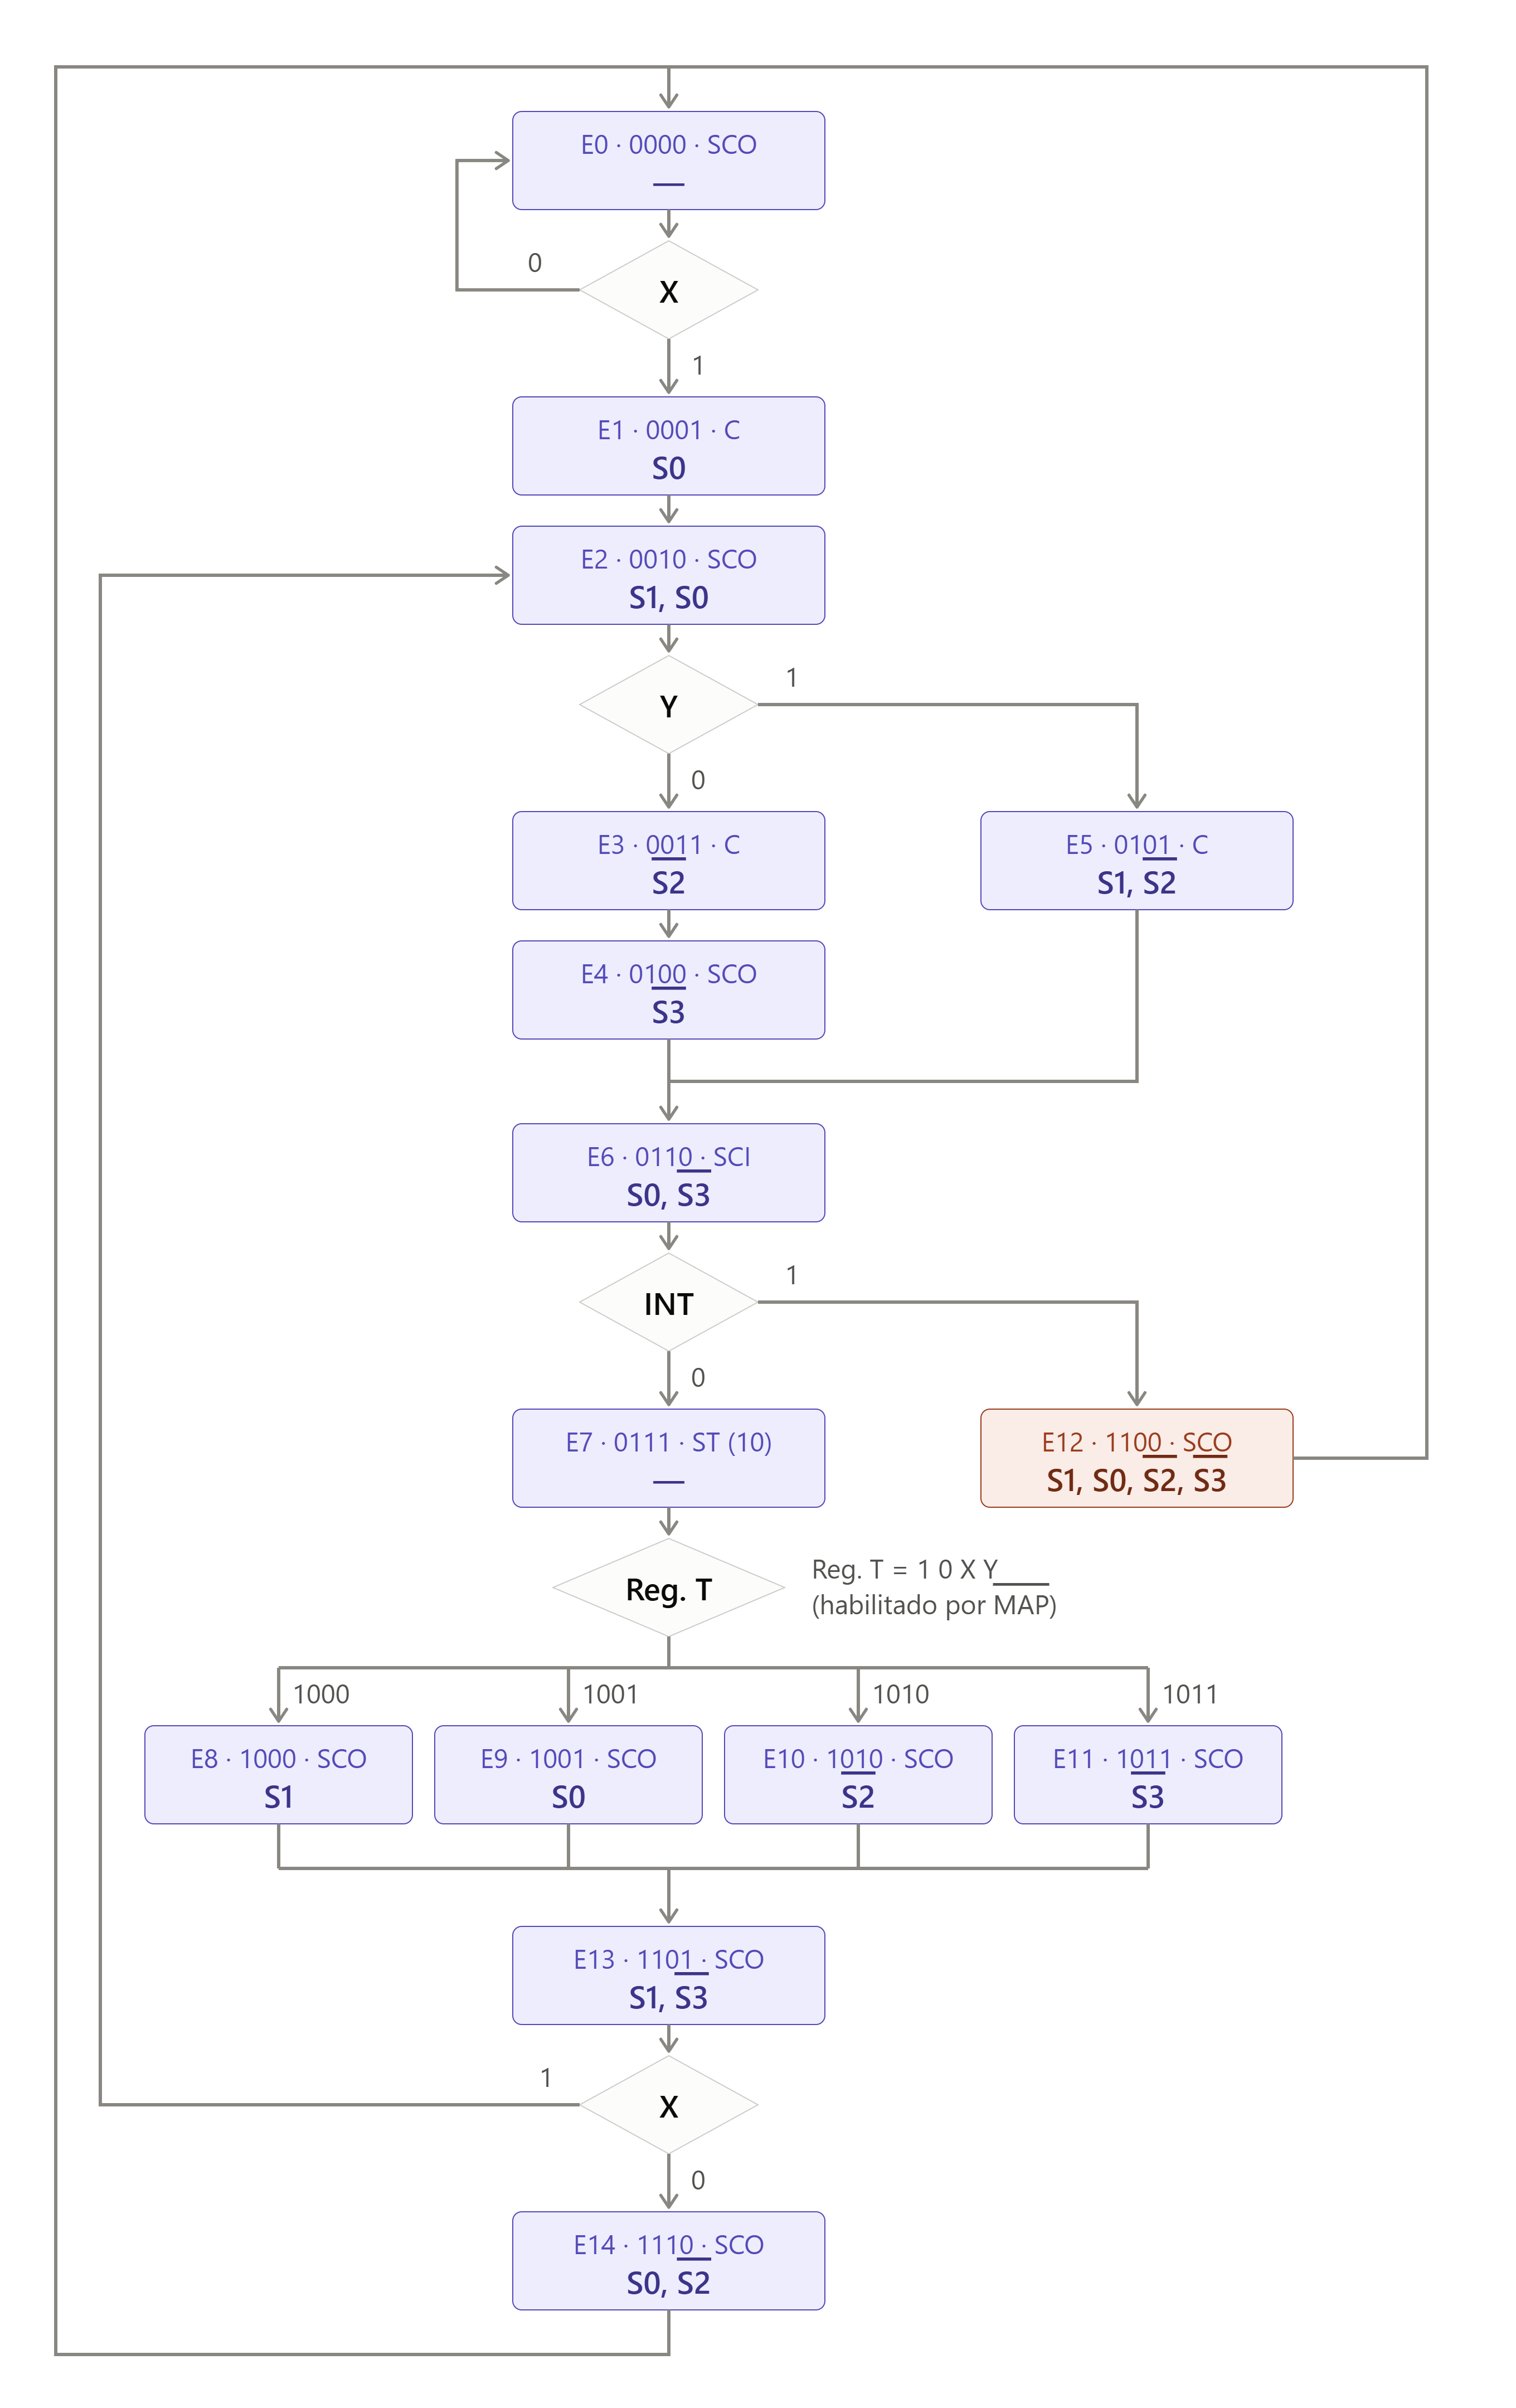
\includegraphics[width=0.78\textwidth]{practica6/evidencias/01-carta-asm.png}
  \caption{Carta ASM del secuenciador básico: 15 estados, entradas X, Y e INT y cuatro salidas.}
  \label{fig:asm}
\end{figure}

Con 15 estados se requieren $\lceil \log_2 15 \rceil = 4$ bits, por lo que hay 16 localidades. La
única localidad sin estado asociado (\texttt{1111}) tiene un contenido de seguridad que regresa a
EST0. La prueba tiene 2 bits: \texttt{00} selecciona X, \texttt{01} selecciona Y, \texttt{10}
selecciona INT y \texttt{11} selecciona una constante en cero (\texttt{aux}), que se usa en las
transiciones incondicionales.

La tabla \ref{tab:entradas} resume la codificación de la prueba.

\begin{table}[H]
  \centering
  \caption{Codificación de la variable sensada en el campo de prueba.}
  \label{tab:entradas}
  \begin{tabular}{@{}c l@{}}
    \toprule
    \textbf{Prueba} & \textbf{Variable} \\
    \midrule
    \texttt{00} & X \\
    \texttt{01} & Y \\
    \texttt{10} & INT \\
    \texttt{11} & \texttt{aux} (constante 0: transición incondicional) \\
    \bottomrule
  \end{tabular}
\end{table}

Las salidas de cada estado se describen con la convención de las prácticas anteriores: en la
memoria se almacena el nivel físico de la señal, de modo que $\overline{S_3}$ y $\overline{S_4}$
valen \texttt{0} cuando están activas.

La carta no tiene salidas condicionales. Las salidas F y V de cada localidad son iguales, por lo
que las salidas dependen sólo del estado presente.

\subsection{Evidencias del laboratorio}

La figura \ref{fig:evid-carta-lab} muestra la carta ASM que se dibujó a mano durante la sesión de
laboratorio, antes de llevarla a la forma digital. Las etiquetas de salida de esa carta usan la
numeración $S_0$ a $S_3$, que corresponde a $S_1$ a $S_4$ en el resto del reporte.

\begin{figure}[H]
  \centering
  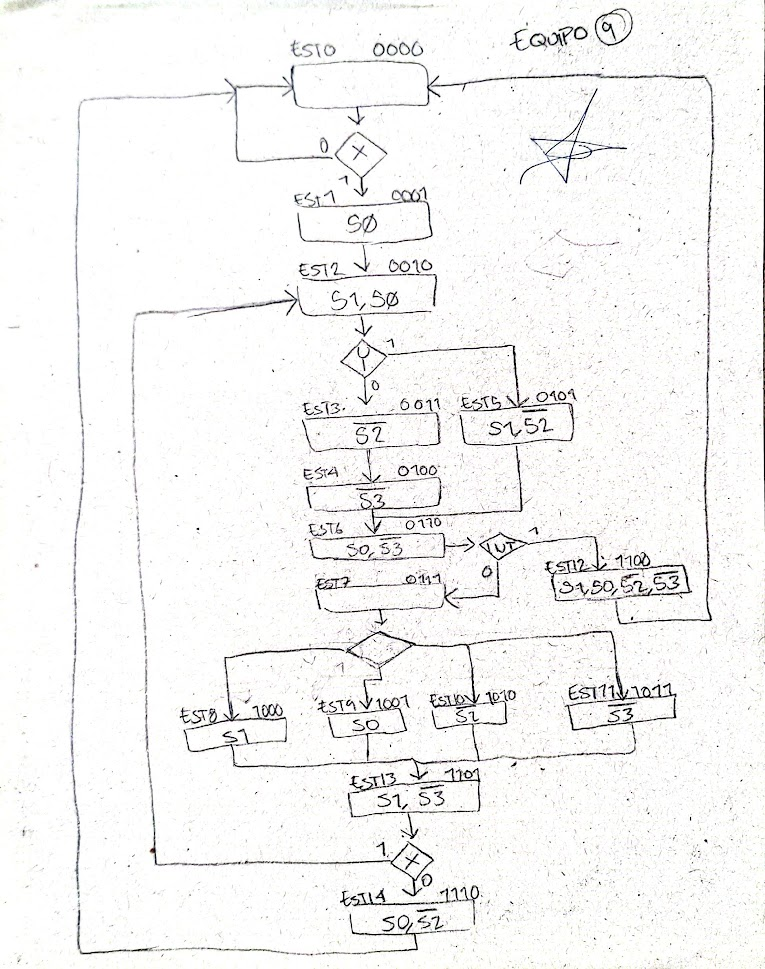
\includegraphics[width=0.9\textwidth,height=0.8\textheight,keepaspectratio]{practica6/evidencias/evidencia-carta-lab.jpg}
  \caption{Carta ASM dibujada durante el laboratorio, con la asignación de códigos de estado.}
  \label{fig:evid-carta-lab}
\end{figure}

La figura \ref{fig:diag-lab} muestra el diagrama de bloques que se armó en Quartus durante el
laboratorio. Es el archivo \texttt{.bdf} que se configuró como entidad de nivel superior.

\begin{figure}[H]
  \centering
  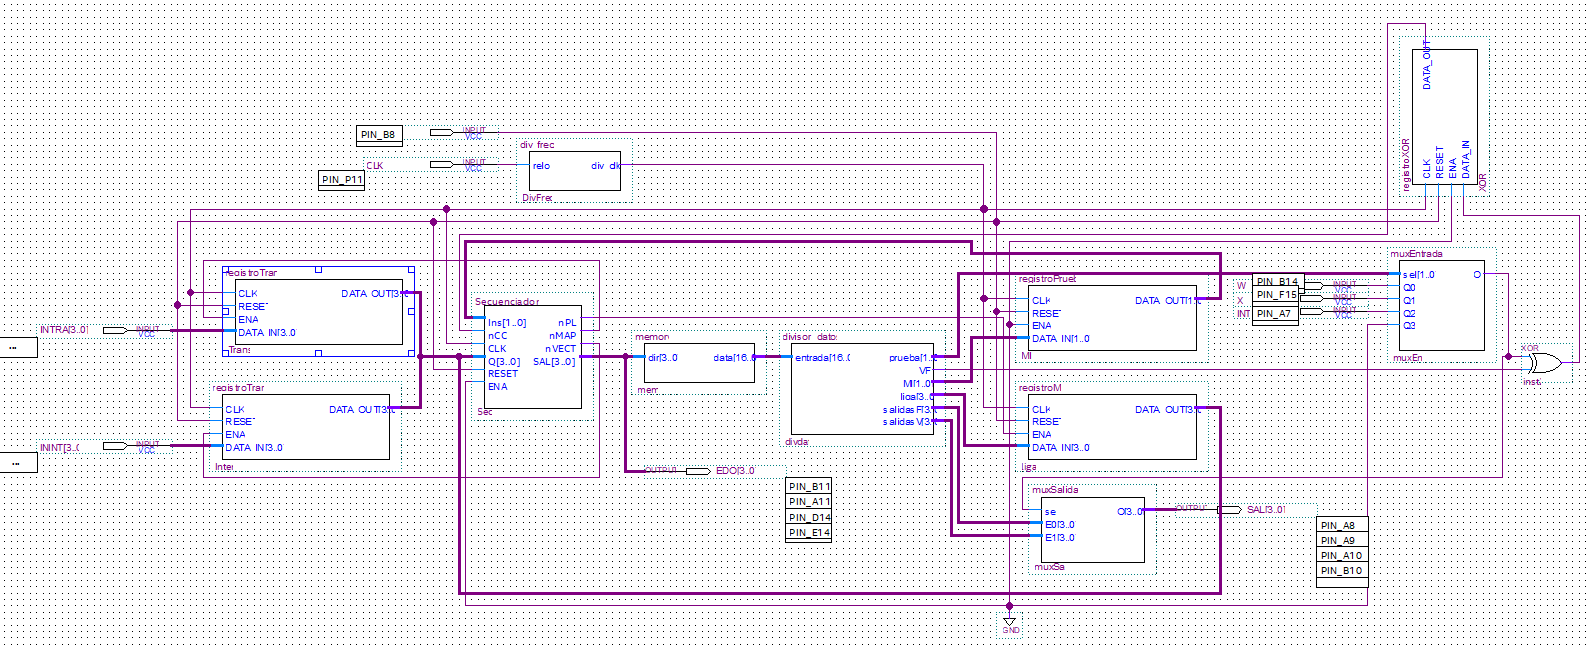
\includegraphics[width=\textwidth]{practica6/evidencias/diagrama-bloques-lab.png}
  \caption{Diagrama de bloques elaborado en el laboratorio (archivo \texttt{.bdf}) del secuenciador básico.}
  \label{fig:diag-lab}
\end{figure}

\subsection{Tamaño de la memoria necesaria}

La dirección se forma con los 4 bits del estado presente, por lo que $n = 4$ y la memoria tiene
$2^4 = 16$ localidades. Cada localidad contiene los siguientes campos:

\begin{center}
\begin{tabular}{@{}l r@{}}
\toprule
\textbf{Campo} & \textbf{Bits} \\
\midrule
Prueba (X, Y, INT, \texttt{aux})      & 2 \\
VF                                    & 1 \\
Microinstrucción (MI)                 & 2 \\
Liga                                  & 4 \\
Salidas F                             & 4 \\
Salidas V                             & 4 \\
\midrule
\textbf{Total} $m$                    & \textbf{17} \\
\bottomrule
\end{tabular}
\end{center}

Por lo tanto

\[
\text{Memoria} = 2^{4} \times 17 = 16 \times 17 = 272 \text{ bits},
\]

es decir, 16 localidades de 17 bits cada una. Quince de ellas corresponden a los estados de la carta
y la localidad \texttt{1111} es de seguridad.

\subsection{Contenido de la memoria}

La palabra se organiza como

\[
\text{dato} = \underbrace{\text{Prueba}}_{(16{:}15)} \ \Vert \
\underbrace{\text{VF}}_{(14)} \ \Vert \
\underbrace{\text{MI}}_{(13{:}12)} \ \Vert \
\underbrace{\text{Liga}}_{(11{:}8)} \ \Vert \
\underbrace{\text{Salidas F}}_{(7{:}4)} \ \Vert \
\underbrace{\text{Salidas V}}_{(3{:}0)}
\]

Dentro de cada campo de salidas, los bits se ordenan como $S_1\, S_2\, \overline{S_3}\, \overline{S_4}$.
La tabla \ref{tab:memoria} presenta las 16 localidades, tal como se escribieron en \texttt{memory.vhd}.

\begin{table}[htbp]
  \centering
  \caption{Contenido de la memoria del secuenciador básico. La dirección 1111 no corresponde a un
  estado de la carta.}
  \label{tab:memoria}
  \small
  \setlength{\tabcolsep}{4pt}
  \begin{tabular}{@{}c c c c c c c c@{}}
    \toprule
    \textbf{Dirección} & \textbf{Estado} & \textbf{Prueba} & \textbf{VF} & \textbf{MI} & \textbf{Liga} & \textbf{Salidas F} & \textbf{Salidas V} \\
    \midrule
    0000 & EST0  & 00 & 0 & 01 & 0000 & 0011 & 0011 \\
    0001 & EST1  & 11 & 0 & 00 & 0000 & 1011 & 1011 \\
    0010 & EST2  & 01 & 1 & 01 & 0101 & 1111 & 1111 \\
    0011 & EST3  & 11 & 0 & 00 & 0000 & 0001 & 0001 \\
    0100 & EST4  & 11 & 0 & 01 & 0110 & 0010 & 0010 \\
    0101 & EST5  & 11 & 0 & 00 & 0000 & 0101 & 0101 \\
    0110 & EST6  & 10 & 1 & 11 & 0000 & 1010 & 1010 \\
    0111 & EST7  & 11 & 0 & 10 & 0000 & 0011 & 0011 \\
    1000 & EST8  & 11 & 0 & 01 & 1101 & 0111 & 0111 \\
    1001 & EST9  & 11 & 0 & 01 & 1101 & 1011 & 1011 \\
    1010 & EST10 & 11 & 0 & 01 & 1101 & 0001 & 0001 \\
    1011 & EST11 & 11 & 0 & 01 & 1101 & 0010 & 0010 \\
    1100 & EST12 & 11 & 0 & 01 & 0000 & 1100 & 1100 \\
    1101 & EST13 & 00 & 1 & 01 & 0010 & 0110 & 0110 \\
    1110 & EST14 & 11 & 0 & 01 & 0000 & 1001 & 1001 \\
    1111 & (sin uso) & 11 & 0 & 01 & 0000 & 0011 & 0011 \\
    \bottomrule
  \end{tabular}
\end{table}

En EST7, la microinstrucción ST entrega la dirección de transformación. Esa dirección se forma con
\texttt{10} y las entradas X e Y, de modo que los cuatro casos llevan a EST8, EST9, EST10 o EST11
según el valor de X e Y.

\subsection{Implementación en VHDL y diagrama de bloques}

El sistema se describió en VHDL y se interconectó en un diagrama de bloques (archivo \texttt{.bdf})
de Quartus, que se configuró como entidad de nivel superior. La figura \ref{fig:bdf} muestra la
interconexión. El secuenciador entrega la dirección \texttt{SAL[3..0]}, que direcciona la memoria.
La palabra leída se separa en prueba, VF, MI, liga y salidas F y V. El selector de entradas
\texttt{muxEntradas} toma la prueba y entrega la variable sensada; la XOR la compara con VF y el
resultado se registra como la condición del secuenciador.

\begin{figure}[H]
  \centering
  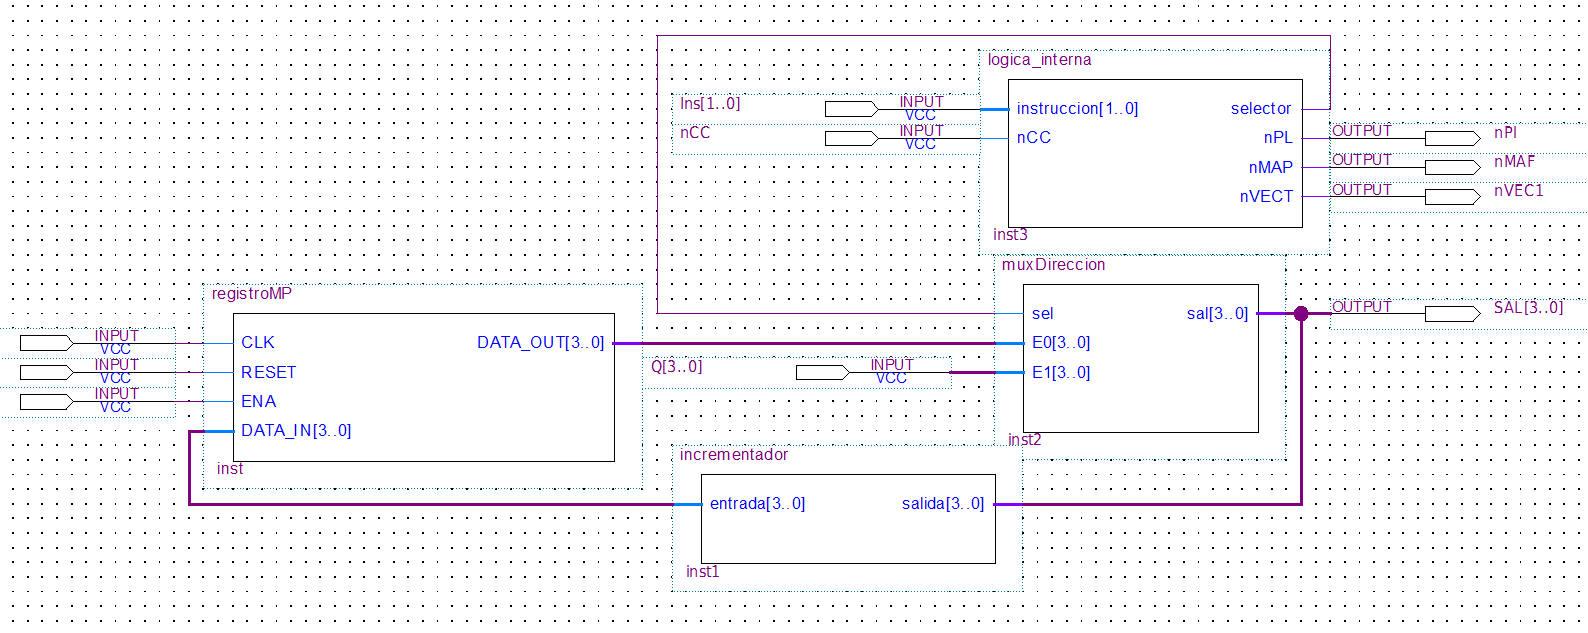
\includegraphics[width=\textwidth]{practica6/evidencias/02-diagrama-bloques.png}
  \caption{Diagrama a bloques de nivel superior (archivo \texttt{.bdf}) del secuenciador básico.}
  \label{fig:bdf}
\end{figure}

El módulo \texttt{memory} implementa la ROM de 16 palabras de 17 bits.

\lstinputlisting[style=hdl]{codigo/memory.vhd}
\captionof{figure}{Código VHDL de la memoria con las 16 localidades del secuenciador básico.}
\label{fig:memory}

El módulo \texttt{divisor\_datos} separa la palabra leída en sus campos.

\lstinputlisting[style=hdl]{codigo/divisor_datos.vhd}
\captionof{figure}{Código VHDL del divisor que separa la palabra en prueba, VF, MI, liga y salidas.}
\label{fig:divisor}

El módulo \texttt{muxEntradas} es el selector de entradas. Su entrada \texttt{Q3} está fija en cero
y permite las transiciones incondicionales.

\lstinputlisting[style=hdl]{codigo/muxEntradas.vhd}
\captionof{figure}{Código VHDL del selector de entradas.}
\label{fig:muxent}

El módulo \texttt{Secuenciador} integra la lógica interna, el multiplexor de dirección, el
incrementador y el registro de microprograma (uPC).

\lstinputlisting[style=hdl]{codigo/Secuenciador.vhd}
\captionof{figure}{Código VHDL del secuenciador básico.}
\label{fig:sec}

La lógica interna decodifica la microinstrucción y genera las señales \texttt{nPL}, \texttt{nMAP} y
\texttt{nVECT}, además de la selección del multiplexor de dirección.

\lstinputlisting[style=hdl]{codigo/logica_interna.vhd}
\captionof{figure}{Código VHDL de la lógica interna que decodifica la microinstrucción.}
\label{fig:logint}

\lstinputlisting[style=hdl]{codigo/muxDireccion.vhd}
\captionof{figure}{Código VHDL del multiplexor de dirección.}
\label{fig:muxdir}

Los registros de liga y de transformación comparten la entrada D del secuenciador mediante salidas
de tres estados. El registro de interrupciones entrega el vector fijo \texttt{1100} (EST12).

\lstinputlisting[style=hdl]{codigo/registroMP.vhd}
\captionof{figure}{Código VHDL del registro de liga.}
\label{fig:regmp}

\lstinputlisting[style=hdl]{codigo/registroTrans.vhd}
\captionof{figure}{Código VHDL de los registros de transformación e interrupciones.}
\label{fig:regtrans}

El módulo \texttt{muxSalidas} selecciona entre las salidas F y V con la variable sensada. Como la
carta no tiene salidas condicionales, ambos conjuntos son iguales en todas las localidades.

\lstinputlisting[style=hdl]{codigo/muxSalidas.vhd}
\captionof{figure}{Código VHDL del selector de salidas.}
\label{fig:muxsal}

Para observar el comportamiento en la tarjeta, un divisor de frecuencia reduce el reloj de 50~MHz a
una frecuencia de transición perceptible.

\lstinputlisting[style=hdl]{codigo/div_frec.vhd}
\captionof{figure}{Código VHDL del divisor de frecuencia.}
\label{fig:divfrec}

\subsection{Asignación de pines}

Para la implementación en la tarjeta DE10-Lite (dispositivo MAX 10 10M50DAF484C7G) se realizó la
asignación de la tabla \ref{tab:pines}. La entrada X se asignó a SW0, Y a SW1 e INT a SW2. El
\textit{reset} se asignó al botón \texttt{KEY0}. Las salidas $S_1$, $S_2$, $\overline{S_3}$ y
$\overline{S_4}$ se asignaron a \texttt{LEDR0} a \texttt{LEDR3}, y el estado presente de 4 bits a
\texttt{LEDR9} a \texttt{LEDR6}.

\begin{table}[H]
  \centering
  \caption{Asignación de pines en la tarjeta DE10-Lite.}
  \label{tab:pines}
  \small
  \begin{tabular}{@{}l l l l@{}}
    \toprule
    \textbf{Señal} & \textbf{Pin} & \textbf{Recurso} & \textbf{Función} \\
    \midrule
    \texttt{CLK}     & \texttt{PIN\_P11} & \texttt{MAX10\_CLK1\_50} & Reloj de 50 MHz \\
    \texttt{RESET}   & \texttt{PIN\_B8}  & \texttt{KEY0}   & \textit{Reset} activo en bajo \\
    \texttt{X}       & \texttt{PIN\_C10} & \texttt{SW0}    & Entrada X \\
    \texttt{Y}       & \texttt{PIN\_C11} & \texttt{SW1}    & Entrada Y \\
    \texttt{INT}     & \texttt{PIN\_D12} & \texttt{SW2}    & Petición de interrupción \\
    \texttt{SAL[3]}  & \texttt{PIN\_A8}  & \texttt{LEDR0}  & Salida $S_1$ (activa en 1) \\
    \texttt{SAL[2]}  & \texttt{PIN\_A9}  & \texttt{LEDR1}  & Salida $S_2$ (activa en 1) \\
    \texttt{SAL[1]}  & \texttt{PIN\_A10} & \texttt{LEDR2}  & Salida $\overline{S_3}$ (activa en 0) \\
    \texttt{SAL[0]}  & \texttt{PIN\_B10} & \texttt{LEDR3}  & Salida $\overline{S_4}$ (activa en 0) \\
    \texttt{EDO[3]}  & \texttt{PIN\_B11} & \texttt{LEDR9}  & Bit 3 del estado presente \\
    \texttt{EDO[2]}  & \texttt{PIN\_A11} & \texttt{LEDR8}  & Bit 2 del estado presente \\
    \texttt{EDO[1]}  & \texttt{PIN\_D14} & \texttt{LEDR7}  & Bit 1 del estado presente \\
    \texttt{EDO[0]}  & \texttt{PIN\_E14} & \texttt{LEDR6}  & Bit 0 del estado presente \\
    \bottomrule
  \end{tabular}
\end{table}

\section{Análisis de resultados}

El proyecto se compiló en Quartus Prime 25.1std Lite Edition sin errores. Antes de programar la
tarjeta se verificó el comportamiento del diseño mediante simulación funcional.

\subsection{Simulación funcional}

La simulación se compiló y ejecutó con GHDL, y la forma de onda se visualizó con GTKWave a partir del
archivo \texttt{sim.vcd}. El \textit{testbench} \texttt{tb\_practica6} instancia la cadena funcional
completa (memoria, divisor de datos, selector de entradas, selectores de salida, secuenciador y
registros) y maneja las entradas X, Y e INT con un reloj de 10~ns. Se omitió el divisor de frecuencia,
porque sólo fija la velocidad perceptible en la tarjeta.

El banco de pruebas aplica 47 pasos que recorren todos los estados de la carta, incluidos los cuatro
saltos de transformación desde EST7 y la rutina de interrupción en EST12. Compara el estado presente
con el esperado en cada paso. Al finalizar reporta: \textit{OK: las 47 transiciones coinciden con la
carta ASM}.

\begin{figure}[H]
  \centering
  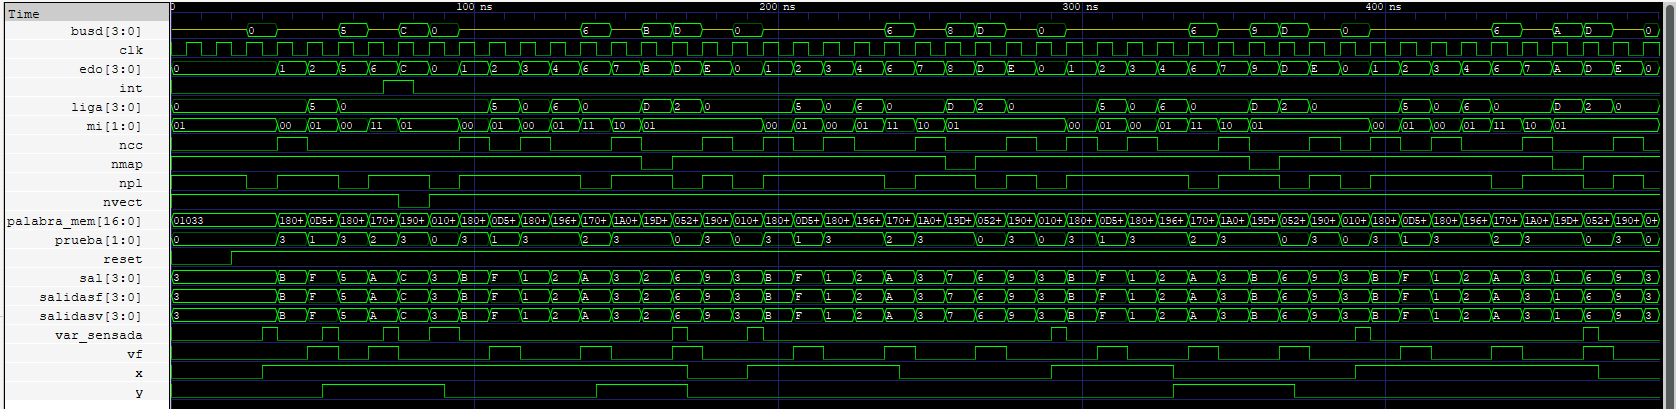
\includegraphics[width=\textwidth]{practica6/evidencias/simulacion.png}
  \caption{Forma de onda de la simulación funcional. Se muestran el reloj, las entradas X, Y e INT,
  el estado presente \texttt{edo}, la palabra leída de memoria, la prueba, VF, la microinstrucción
  \texttt{mi}, la liga, las señales de habilitación, la condición y las salidas.}
  \label{fig:sim}
\end{figure}

En la figura se observa que el estado presente recorre la secuencia de la carta. Las señales de
habilitación \texttt{nPL}, \texttt{nMAP} y \texttt{nVECT} se activan en los pasos que corresponden
a cada tipo de salto.

\subsection{Verificación en la tarjeta}

Se programó la DE10-Lite con el diseño y se comprobó su funcionamiento en el laboratorio. La máquina
recorrió los estados de la carta conforme a las entradas X, Y e INT, incluidos el salto a la
rutina de interrupción y los saltos de transformación. El funcionamiento se mostró a la profesora
durante la sesión, y la máquina respondió correctamente.

\section{Conclusiones individuales}

\subsection{Omar Alfonso Zendejas Labias}

Con esta práctica entendí cómo un secuenciador controla una máquina de estados sin necesidad de
una liga distinta para cada decisión. La microinstrucción de cada localidad decide si el siguiente
estado es el contiguo, el de la liga, el de transformación o el vector de interrupción, y el
multiplexor de dirección es el que une esos orígenes. Lo que más me sirvió fue ver que registrar la
microinstrucción y la condición antes de usarlas evita que el lazo sea puramente combinacional.

\subsection{Emiliano García Olvera}

Considero que el objetivo de la práctica se cumplió. Se construyó un secuenciador básico para una
máquina de 15 estados, con una memoria de 16 localidades de 17 bits, es decir, 272 bits en total
(tabla \ref{tab:memoria}). La simulación con los 47 pasos del testbench no presentó discrepancias,
y en la tarjeta la máquina respondió de acuerdo con la carta, incluido el salto a la rutina de
interrupción. Lo que más me aportó la práctica fue entender que las transformaciones de un estado
a varios destinos, como EST7, se resuelven con una dirección formada por las entradas, sin ocupar
una liga por cada caso.

\renewcommand{\refname}{Bibliografía}
\begin{thebibliography}{9}
\bibitem{savage} J. Savage Carmona, G. Vázquez y N. E. Chávez Rodríguez,
  \emph{Diseño de microprocesadores}. Ciudad de México, México: Facultad de Ingeniería,
  Universidad Nacional Autónoma de México, 2017. [En línea]. Disponible:
  \url{http://profesores.fi-b.unam.mx/luist/archivos/MicroprocesadoresSavage.pdf}
\end{thebibliography}

\end{document}